%%%%%%%%%%%%%%%%%%%%%%%%%
%% Document and Layout %%
%%%%%%%%%%%%%%%%%%%%%%%%%

% Fix for multiple "No room for a new \dimen" errors.
%
% See: http://tex.stackexchange.com/questions/38607/no-room-for-a-new-dimen
%
\usepackage{etex}

\usepackage[utf8]{inputenc}

% Fix for "'babel/polyglossia' detected but 'csquotes' missing"
% warning. NOTE: Include after inputenc.
%
\usepackage{csquotes}

% Make internal macro definitions accessible,
% e.g. \@title, \@date \@author.
\makeatletter

% Multi-column support.
\usepackage{multicol}

% A useful package which includes macros like \ifdef{}{}{}:
%
\usepackage{etoolbox}

% Uncomment the following line to remove column separation:
%
%\setlength{\columnsep}{5mm}

% Allow user-defined warning and error filters.
%
\usepackage{silence}


%%%%%%%%%%%%%%%%%%%%%
% Table of Contents %
%%%%%%%%%%%%%%%%%%%%%

% % Set chapter and section numbering depth:
% %
% \setcounter{secnumdepth}{2}


%%%%%%%%%%%%%%%%
% Bibliography %
%%%%%%%%%%%%%%%%
\usepackage[%
    backend=biber,
    style=numeric-comp,
    % style=numeric-comp,  % numerical-compressed
    sorting=none,        % nty,nyt,nyvt,anyt,anyvt,ynt,ydnt,none
    sortcites=true,      % sort \cite{b a d c}: true,false
    block=none,          % space between blocks: none,space,par,nbpar,ragged
    indexing=false,      % indexing options: true,false,cite,bib
    citereset=none,      % don't reset cites
    isbn=false,          % print ISBN?
    url=true,            % print URL?
    doi=false,           % print DOI?
    natbib=true,         % natbib compatability
  ]{biblatex}

% % Filter annoying and unavoidable biblatex warning:
\WarningFilter{biblatex}{Patching footnotes failed}

% Reduce the font size of the bibliography:
% \renewcommand{\bibfont}{\normalfont\scriptsize}

% Determine which BibTeX file to use:
%
% If available, use my Mendeley BibTex library, located in the home
% directory. Note that this is a relative path and will break if
% either this file or the BibTex library are moved. If the library is
% not present, use the local refs.bib file.
\newcommand{\BibResourceGlobal}{../../library.bib}
\newcommand{\BibResourceLocal}{refs.bib}

\IfFileExists{\BibResourceGlobal}
  {\newcommand{\BibResource}{\BibResourceGlobal}}
  {\newcommand{\BibResource}{\BibResourceLocal}}

\addbibresource{\BibResource}


%%%%%%%%%%%%%%
% Appendices %
%%%%%%%%%%%%%%

% Appendix package. Documentation:
%
%  http://mirror.ox.ac.uk/sites/ctan.org/macros/latex/contrib/appendix/appendix.pdf
%
% Package options:
%
% toc      - Put a header (e.g., `Appendices') into the Table of Contents
%            (the ToC) before listing the appendices. (This is done by
%            calling the \addappheadtotoc command.)
% page     - Puts a title (e.g., `Appendices') into the document at the
%            point where the appendices environment is begun. (This is
%            done by calling the \appendixpage command.)
% title    - Adds a name (e.g., `Appendix') before each appendix title in
%            the body of the document. The name is given by the value
%            of \appendixname. Note that this is the default behaviour
%            for classes that have chapters.
% titletoc - Adds a name (e.g., `Appendix') before each appendix listed
%            in the ToC. The name is given by the value
%            of \appendixname.
% header   - Adds a name (e.g., `Appendix') before each appendix in page
%            headers.  The name is given by the value
%            of \appendixname. Note that this is the default behaviour
%            for classes that have chapters.
\usepackage[title, titletoc]{appendix}


%%%%%%%%%%%%%%%%%%%%%%%%%%%%%%%%%%%%%
%% Figures, footnotes and listings %%
%%%%%%%%%%%%%%%%%%%%%%%%%%%%%%%%%%%%%

%\usepackage{float}
%\restylefloat{figure}

% Use bold ``(Figure|Table|Listing)'' caption text.
%\usepackage[margin=1cm]{caption}

% Set the font for captions.
% \renewcommand{\captionfont}{\small}
% Set the font for caption labels.
% \renewcommand{\captionlabelfont}{\footnotesize\bf}

% Use arabic numbers for footnote.
%\renewcommand{\thefootnote}{\arabic{footnote}}

% Ensure that footnotes always appear at the bottom of pages.
%\usepackage[bottom]{footmisc}

% Reset the footnote counter on every page.
%\usepackage{perpage}
%\MakePerPage{footnote}

% Pre-requisites for rendering upquotes in listings package.
\usepackage[T1]{fontenc}
\usepackage{lmodern}
\usepackage{textcomp}

% Pseudo-code listings.
\usepackage{algorithm}
\usepackage{algpseudocode}
\newcommand{\Break}{\State \textbf{break} }
\algblockdefx[Loop]{Loop}{EndLoop}[1][]{\textbf{Loop} #1}{\textbf{End
    Loop}}

\algrenewcommand\ALG@beginalgorithmic{\footnotesize}

% Code listings.
\usepackage{listings}

% Set \ttfamily to use courier fonts.
%
% See: http://tex.stackexchange.com/a/33686
%
\usepackage{courier}

\lstset{frame=bt,                    % Add top and bottom frame lines
        breaklines=true,             % Force line wrapping
        captionpos=b,                % Place caption below listing
        numbers=left,                % Add left-side line numbers
        basicstyle=\scriptsize\ttfamily, % Set font size and type
        showstringspaces=false,      % Don't show visible whitespace
        numberstyle=\tiny,
        upquote=true,                % Use upright quotes, not curly
        commentstyle=\bfseries}      % Embolden comments

% Use (*@ @*) to escape LaTeX commands within listings.
\lstset{escapeinside={(*@}{@*)}}

% Add 10pt space between chapters in TOC listings entries:
%\let\Chapter\chapter
%\def\chapter{\addtocontents{lol}{\protect\addvspace{10pt}}\Chapter}


%%%%%%%%%%%%%%%%%%%%%%%%
%% Graphics and maths %%
%%%%%%%%%%%%%%%%%%%%%%%%
\usepackage{amsmath}

% Vector notation, e.g. \vv{x}:
%
\usepackage{esvect}

% Additional amsmath symbols, see:
%
% http://texblog.org/2007/08/27/number-sets-prime-natural-integer-rational-real-and-complex-in-latex/
%
\usepackage{amsfonts}
\usepackage{amssymb}

\usepackage{graphicx}
\usepackage{mathtools}
\usepackage{tikz}
\usepackage{tikz-qtree}

% Provide bold font face in maths.
\usepackage{bm}

\usepackage{subcaption}
\expandafter\def\csname ver@subfig.sty\endcsname{}

% Define an 'myalignat' command which behave as 'alignat' without the
% vertical top and bottom padding. See:
%     http://www.latex-community.org/forum/viewtopic.php?f=5&t=1890
\newenvironment{myalignat}[1]{%
  \setlength{\abovedisplayskip}{-.7\baselineskip}%
  \setlength{\abovedisplayshortskip}{\abovedisplayskip}%
  \start@align\z@\st@rredtrue#1
}%
{\endalign}

% Define additional operators:
\DeclareMathOperator*{\argmin}{arg\,min}
\DeclareMathOperator*{\argmax}{arg\,max}

\DeclareMathOperator*{\gain}{Gain}

% Skeleton operators.
\DeclareMathOperator*{\map}{Map}
\DeclareMathOperator*{\reduce}{Reduce}
\DeclareMathOperator*{\scan}{Scan}
\DeclareMathOperator*{\stencil}{Stencil}
\DeclareMathOperator*{\zip}{Zip}
\DeclareMathOperator*{\allpairs}{All\,Pairs}

% Maths plots using pgfplots, see:
%
%     http://pgfplots.sourceforge.net/pgfplots.pdf
%
\usepackage{pgfplots}

% Disable compatability mode.
%
\pgfplotsset{compat=1.12}

% Gantt charts using pgfgantt, see:
%
%     http://www.ctan.org/pkg/pgfgantt
%
\usepackage{pgfgantt}

% Fix milestone aspect ratio by defining a custom element.
\newganttchartelement*{mymilestone}{
  mymilestone/.style={
    shape=diamond,
    inner sep=2pt,
    draw=black,
    top color=black,
    bottom color=black,
  }
}

% Tikz flowchart configuration.
\usetikzlibrary{shapes,arrows,shadows,fit,backgrounds}
\tikzstyle{decision} = [diamond,
                        draw,
                        text width=4.5em,
                        text badly centered,
                        node distance=3cm,
                        inner sep=0pt]
\tikzstyle{block}    = [rectangle,
                        draw,
                        text width=5em,
                        text centered,
                        node distance=3cm,
                        minimum height=4em,
                        inner sep=.2cm]
\tikzstyle{line}     = [draw, -latex']

% Add dirtree picture style, see:
%
%     http://tex.stackexchange.com/a/34268
%
\newcount\dirtree@lvl
\newcount\dirtree@plvl
\newcount\dirtree@clvl
\def\dirtree@growth{%
  \ifnum\tikznumberofcurrentchild=1\relax
    \global\advance\dirtree@plvl by 1
    \expandafter\xdef\csname dirtree@p@\the\dirtree@plvl\endcsname{\the\dirtree@lvl}
  \fi
  \global\advance\dirtree@lvl by 1\relax
  \dirtree@clvl=\dirtree@lvl
  \advance\dirtree@clvl by -\csname dirtree@p@\the\dirtree@plvl\endcsname
  \pgf@xa=0.33cm\relax
  \pgf@ya=-\baselineskip\relax
  \pgf@ya=\dirtree@clvl\pgf@ya
  \pgftransformshift{\pgfqpoint{\the\pgf@xa}{\the\pgf@ya}}%
  \ifnum\tikznumberofcurrentchild=\tikznumberofchildren
    \global\advance\dirtree@plvl by -1
  \fi
}
\tikzset{
  dirtree/.style={
    growth function=\dirtree@growth,
    every node/.style={anchor=north},
    every child node/.style={anchor=west},
    edge from parent path={(\tikzparentnode\tikzparentanchor) |- (\tikzchildnode\tikzchildanchor)}
  }
}

% UML sequence diagram macros, see:
%
%     https://code.google.com/p/pgf-umlsd/
%
% Options:
%
%     underline - Underline object names
%
\usepackage[underline=false]{pgf-umlsd}

% Support for SVG graphics.
%
% NOTE that you must pass the "--shell-escape" argument to pdflatex to
% compile. NOTE also that images *MUST* be placed within the graphics
% path.
\usepackage{svg}
\graphicspath{{img/}}

%%%%%%%%%%%%%%%%%%%%%%
%% Tables and lists %%
%%%%%%%%%%%%%%%%%%%%%%

% Required to use labm8 exported tables.
%
\usepackage{booktabs}

% Required for full page-width tables.
\usepackage{tabularx}

%\usepackage{enumitem}
%\setenumerate{itemsep=0pt}

% Use no left margin for lists:
%\setlist{leftmargin=*}

\usepackage{longtable}

% Define column types L, C, R with known text justification and fixed
% widths:
\usepackage{array}
\newcolumntype{L}[1]{>{\raggedright\let\newline\\\arraybackslash\hspace{0pt}}m{#1}}
\newcolumntype{C}[1]{>{\centering\let\newline\\\arraybackslash\hspace{0pt}}m{#1}}
\newcolumntype{R}[1]{>{\raggedleft\let\newline\\\arraybackslash\hspace{0pt}}m{#1}}


%%%%%%%%%%%%%%%%%%%%%%%%%%%%%
%% Typesetting and symbols %%
%%%%%%%%%%%%%%%%%%%%%%%%%%%%%

% Adjustable font sizes in \Verbatim{}
\usepackage{fancyvrb}

%\usepackage{titlesec}
% Set section and paragraph heading fonts:
%\titleformat*{\section}{\Large\bfseries}
%\titleformat*{\subsection}{\normalsize\bfseries}
%\titleformat*{\subsubsection}{\normalsize}
%\titleformat*{\paragraph}{\large\bfseries}
%\titleformat*{\subparagraph}{\large\bfseries}

% Set section heading margins. Usage:
% \titlespacing*{<command>}{<left>}{<before>}{<after>}
%\titlespacing*{\section}{0pt}{.6em}{.3em}
%\titlespacing*{\subsection}{0pt}{.6em}{.2em}

% Set paragraph indentation size. Default is 15pt.
%\setlength{\parindent}{10pt}

% The line spacing can be globally set using \linespread:
%
% \linespread{1.2}

% Add a command \hr{} which will draw a horizontal rule the width of
% the text.
%
\newcommand{\hr}{\noindent\makebox[\linewidth]{\rule{\textwidth}{0.2pt}}}

% Add a command \br{} which will create a horizontal space of exactly
% one line height.
%
\newcommand{\br}{\hspace{\baselineskip}}

% Define a command to allow word breaking.
\newcommand*\wrapletters[1]{\wr@pletters#1\@nil}
\def\wr@pletters#1#2\@nil{#1\allowbreak\if&#2&\else\wr@pletters#2\@nil\fi}

% Define a command to create centred page titles.
\newcommand{\centredtitle}[1]{
  \begin{center}
    \large
    \vspace{0.9cm}
    \textbf{#1}
  \end{center}}

% Support hyperlinks using the \hyperref, \url and \href
% macros. Usage:
%
%    \hyperref[label_name]{''link text''}
%
%    \url{<my_url>}
%
%    \href{<my_url>}{<description>}
%
\usepackage{hyperref}

% Disable colored borders of links, cross-references etc in PDF output
\hypersetup{pdfborder={0 0 0}}

% Provide generic commands \degree, \celsius, \perthousand, \micro
% and \ohm which work both in text and maths mode.
\usepackage{gensymb}

%%%%%%%%%%%%%%%%%%%%%%%%%%%%%%%%%
%% Placeholder text generation %%
%%%%%%%%%%%%%%%%%%%%%%%%%%%%%%%%%

% Use either \blindtext or \libpsum to generate placeholder text. Also
% note the macros \blinditemize, \blindenumerate, \blinddescription.
\usepackage[english]{babel}
\usepackage{blindtext}
\usepackage{lipsum}


\begin{document}

\title{Plausible Test Case Generation for Identifying Compiler and Runtime Bugs}

%
% any author declaration will be ignored  when using 'pldi' option (for double blind review)
%
\authorinfo{Person 1 \and Person 2}
{\makebox{A Department} \\
        \makebox{A University}  \\
        \makebox{A Place, AS 12345}}
{\{person1,person2\}@cs.auniv.edu}

\maketitle

\begin{abstract}
%We introduce DeepSmith, a novel approach to the compiler validation problem. While prior works require expert domain knowledge to craft random program generators from probabilistic grammars or program mutation, we instead frame the generation of random programs a language modeling problem. We apply deep learning techniques over millions of lines of handwritten code in order to automatically construct models capable of generating plausible, human-like code samples.

% Our approach complements the desires of compiler developers, who desire small test cases based on ``plausible'' language constructs.
\vspace{2mm}
Compilers should produce correct code for valid inputs, and meaningful errors for invalid inputs. Failure to do so can hinder software development or even cause catastrophic runtime errors. Still, properly testing compilers is hard. Manually assembled test suites cannot cover the enormous range of possible inputs. %
%
% Random program generators come close to it but they require extensive development effort for every language supported by the compiler, and often leave parts of the language space untested. A better way for testing compilers is needed.
% 
Random program generation --- fuzzing --- is an effective technique for discovering bugs in compilers but successful program generators require extensive development effort for every language supported by the compiler, and often leave parts of the language space untested. A better way for testing compilers is needed.

% A novel approach for the rapid development of broad, undirected fuzzers
We introduce DeepSmith, a novel approach which takes advantage of state-of-the-art deep learning techniques to automate and accelerate compiler validation. Our approach constructs a learned model of the structure of real world code based on a large corpus of open source code. Then, it uses the model to automatically generate tens of thousands of realistic programs. Finally, it applies established differential testing methodologies on them to expose bugs in compilers.

We apply our approach to the OpenCL programming language, automatically exposing bugs in OpenCL compilers with little effort on our side. In 1,000 hours of automated testing of commercial and open source compilers, we discover bugs in all of them, %
%
% made up of XX interesting test cases, compared to a similar XX for the state of the art technique given the same time.
%
submitting \todo{67} bug reports.
%
Our test cases are on average two orders of magnitude smaller than the state-of-the-art, require $3.03\times$ less time to generate and evaluate, and expose bugs which have not been found using existing techniques. Our random program generator, comprising only 500 lines of code, took 14 hours to train for OpenCL versus the state-of-the-art taking 9 man months to port from a generator for C and 50,000 lines of code.
% find CLSmith/src -name '*.cpp' -o '*.h' | xargs wc -l  # 49775

%Compilers should produce correct code for valid inputs, and produce meaningful errors when inputs are invalid. Fixed test-suites and formal verification techniques cannot ensure these properties over the enormous range of possible inputs and complexity of optimizing compilers, leading to the development of random program generators that attempt to find compiler bugs by comparing the outputs of programs across compilers.

%Grammar-based random program generators require extensive development effort, and by design, yield large, ``implausible''  programs which bare little resemblance to actual real code written by human programmers. This is in contrast to the needs of compiler developers, who desire small test cases which are symptomatic of  ``plausible'' use cases. What is needed is a technique for biasing the production of random program generation such that they more closely resemble real handwritten code, and which expose bugs which are likely to arise from common use cases.

% Furthermore, extensive effort is expended on minimizing the risk of undefined behavior, which comes at the cost of reduced expressiveness.

%We introduce DeepSmith, a novel approach to the compiler validation problem. By framing the generation of random programs as a language modeling problem, we apply deep learning techniques over large corpuses of open source codes to learn models which describe the structure of real world codes. We use these models to generate tens of thousands of new programs, and show how established differential testing methodologies can be used to expose bugs in compilers which are symptomatic of real hand-written code.

%We apply our technique to OpenCL, automatically exposing bugs in OpenCL compilers which are likely to arise from real world use cases, in a ways which are not possible using existing techniques. In over 1,000 hours of automated testing of commercial and open source compilers, we discover bugs in all of them, submitting XX bug reports. Our test cases are on average two orders of magnitude smaller than the state-of-the-art, require $3.03\times$ less time to generate and evaluate, and expose bugs which have not be found using existing techniques. \cc{TODO: complimentary approach}

% Our paper serves two purposes: first, we propose a novel methodology for compiler test case generation, capable of finding bugs at a faster rate and covering more areas of the compiler than existing approaches; second, we report on the state of OpenCL implementations.
\end{abstract}


\section{Introduction}\label{sec:intro}

\cc{Chris comment}
\pp{Pavlos comment}
\am{Alastair comment}
\hl{Hugh comment}

\begin{figure}
  \centering
  \includegraphics[width=.85\columnwidth]{img/difftest} %
  % \vspace{-2em}%
  \caption{%
    Differential testing a single test case across multiple testbeds. A test case consists of a program source and its runtime parameters and data. % Outcomes may be the output of the program execution, a compiler crash, a runtime crash, or a timeout error.%
  }%
  \label{fig:difftest}
\end{figure}

\noindent
Optimizing compilers are large and complex programs, with a practically infinite scope of possible inputs. Fixed test-suites are inadequate for ensuring correct behavior over such a range of inputs, and the lack of formal specifications for sections of compilers renders formal verification unusable beyond isolated subcomponents. Yet, compilers are a fundamental trusted technology, and identifying their bugs is of critical importance.

% XSmith: It is difficult to create effective fuzzers for programming language compilers and interpreters because these systems have highly structured inputs, but it is important that such fuzzers exist. Programming language implementations are critical software infrastructure: defects in compilers and interpreters can potentially have great costs in terms of software correctness and reliability, human productivity, and computer security. This project seeks to reduce the time and human effort needed to create sophisticated fuzzers for programming language implementations. In so doing, this project is expected to advance the state of the art in random software testing, improve the quality of several programming language implementations selected for study, and produce new open-source software tools that programmers can use to develop new and more effective fuzz testers.

Differential Testing is an effective and widely studied methodology for identifying compiler bugs~\cite{Chen2014a,Kossatchev2005,Chen2013}. Figure~\ref{fig:difftest} shows the approach. A program and a set of inputs, henceforth referred to as a \emph{test case}, is compiled and executed multiple \emph{testbeds}. If any of the compilers crash or loop indefinitely, or if the output of the programs differs between compilers, then a potential bug has been discovered. \cc{TODO: Early work in context free grammar enumeration to text syntax analyzers~\cite{Purdom1972,Malloy2001}. These can't test past the compiler front-end. Early program generators~\cite{Zhao2009},\cite{Bryan2007}. Now, CSmith~\cite{Yang2011} and EMI testing~\cite{Le2013a} enable deeper, middle-end testing.}

A probabilistic grammar is used to enumerate a large, random program, which is then compiled and executed across a number of compilers. In this manner, CSmith~\cite{Yang2011}, a random program generator for the C programming language, has been used to identify hundreds of bugs in compilers. CSmith defines a probabilistic grammar over a large subset of the C programming language, and recursively instantiates a program, using rigorous and conservative static and dynamic analysis to ensure that programs are free from undefined behavior.

Developing a random program generation is a huge undertaking, requiring a thorough understanding of the target programming language --- CSmith was developed over the course of years, and consists of over 40k lines of handwritten C++ code. By tightly coupling the generation logic with the target programming language, each feature of the grammar must be painstakingly and expertly engineered, and is accompanied by exponential costs in developing the static and dynamic safety checks to ensure that generated programs remain free from (or at least, are likely free from) undefined behavior. For example, lifting CSmith from C to OpenCL~\cite{Lidbury2015a} took 9 months and 8k lines of code. As such, typically only a subset of the language is implemented, and the expressiveness of the grammar is bounded by the limits of static and dynamic analysis. \cc{exhaustive testing is impossible - requiring enumeration of every sequence of characters, but grammar enumeration leaves too many bugs on the table.? }
% --- to date, important language features such as strings, dynamic memory allocation, function pointers, and recursion are unsupported.
% , despite the large overlap between C and OpenCL (which is C with extensions). This huge development cost is extended to the reduction tools too, with CLReduce~\cite{Pflanzer2016} requiring extensions to OCLgrind.

\cc{What is needed\ldots}

We present a novel, data-driven approach to the generation of random programs for compiler fuzzing. Using a corpus of handwritten code in a particular programming language, we use deep neural networks to automatically construct probabilistic models for how humans write programs. The neural networks, without prior knowledge, infer both the syntax and semantics of the programming language, and the common constructs and patterns. By framing the generation of random programs as a language modeling problem, we greatly simplify the process of program generation, and the expressiveness of generated programs is limited only by what is contained in the corpus. Such corpuses can readily be assembled from open source repositories.

\cc{TODO: syntactic modeling trade-off}

Our implementation, DeepSmith, targets OpenCL, an open standard for programming heterogeneous systems, though our approach is language agnostic. We chose OpenCL for three reasons: it is an emerging standard with the challenging promise of portability across a diverse range of heterogeneous hardware; OpenCL is compiled ``online'', meaning that compiler defects may not be discovered until a product is deployed to customers; and OpenCL is a hard programming language to test --- the data-parallel programming model increases the complexity of static and dynamic analysis, further limiting the expressiveness of grammar-based approaches.

%The importance of sane compiler behavior is amplified for OpenCL since it is compiled online. OpenCL code is shipped by developers to customers for compilation online. OpenCL is increasingly used in safety critical software products such as automotive vision. Segmentation faults and other runtime crashes during online compilation can disrupt the execution of safety critical processes.
%
%By design, the grammar-based approach specifically targets the compiler middle-end. Prior work \cite{McKeeman1998}
%
%This approach focuses the
%
%CSmith~\cite{Yang2011}, a popular random program generator for the C programming language, defines a probabilistic grammar over a large subset of the C programming language, and recursively instantiates a program, using rigorous and conservative static and dynamic analysis to ensure that programs are free from undefined behavior.
%
%Typically, these generated programs are many hundreds or thousands of lines long. As such, an additional test case reduction process is usually required, iteratively mutating the program in an attempt to produce a minimal working example which preserves the behavior of interest.
%
%--- to date, CLSmith does not support unions, dynamic memory allocation, strings, etc. EMI testing can simplify the production somewhat by reducing the generation only to program mutations, and deadcode insertions, but \ldots.
%
%Our observations are twofold: such rigorous and conservative methods may be artificially limiting, and that the wealth of code on the web can be used to seed the generation of codes. This paper describes our experiences in using the latter to test OpenCL.
%
%Because Csmith programs are free form undefined behavior, there is only a single interpretation. This allows oracle-less differential testing across compilers, using a voting heuristic to identify erroneous compiler outputs.
%
%Developing a random program generator is a huge undertaking, requiring expert knowledge of the target programming language. CSmith~\cite{Yang2011} was developed over a period of years, and consists of over 40k lines of hand-written C++. CSmith interleaves static analysis with code generation, and inserts runtime checks for cases where static analysis is inadequate. The ``shape'' of CSmith programs is dictated by 80 probabilities; these were extensively hand tuned so that programs ``look right''. Beyond this, the expressiveness of CSmith-generated programs is
%
%\cc{We propose \ldots}
%
%In contrast to probabilistic grammar-based approaches, our approach is programming language agnostic, requiring only a corpus of sample programs in the intended programming language. Such corpuses can be readily be assembled from GitHub. We then use state-of-the-art deep learning techniques to automatically infer the semantics and common usage of a programming language. Learning and sampling an LSTM model requires less than a 100 line of Python script, and contains no programming language-specific logic. The expressiveness of synthesized programs is governed by the corpus; unlike with grammar-based approach, in which every new language feature must be engineered. E.g. to date, CSmith does not support floating points, unions, strings, dynamic memory allocation, function pointers, or recursion. Additionally, all integer arithmetic is wrapped in ``safe math'' macros.
%
%We also, for the first time, provide a means of testing compiler behaviour under plausibly-invalid input conditions. We generate plausible but ill-formed inputs. Prior work used random ASCII sequences to identify compiler front-end bugs~\cite{McKeeman1998}. By mimicking hand written code, our technique is capable of discovering bugs further within the compiler, including middle-end and even code generation.
%
%The design trade-off of our approach is that unstructured, syntactic-level synthesis of program code removes the guarantee that programs are free from undefined behavior, a property which previous approaches have relied upon. In practice, we found this requirement to be too conservative. In testing XXX cases, we discovered only XX cases where a program without a single interpretation was not trivially detectable through differential testing and presented a false positive.
%% Reference: UB in C https://blog.regehr.org/archives/1520
%% Reference: C99 spec appendix J2 - list of UBs
%% OpenCL un-undefines some of those behaviours (e.g. it provides conversion functions between data types), but also adds to them.

% \noindent
We make the following contributions:
%
\begin{itemize}
\item A novel, data-drive approach for the generation of expressive random programs for compiler fuzzing. DeepSmith \emph{infers} programming language use from real-world examples in order to generate plausible compiler test cases; % CLSmith requires expert-driven development for every language feature supported. 40+k lines of C++ vs a few hundred lines of Python.
\item through syntactic modeling of handwritten program code we discover bugs in compilers which the grammar-based approaches cannot, covering more components of the compiler;
% e.g. ill-formed
\item we find bugs faster than the state-of-the-art. In 48 hours we discovered and report XX bugs in compiler and open source OpenCL implementations, XX\% more than CLSmith over the same time period;
\item in modeling real handwritten code, our test cases are more interpretable than other approaches. Average test case size is two orders of magnitude smaller than state-of-the-art;
\end{itemize}

\section{Motivation}\label{sec:methodology}

\newsavebox{\IntelSizetIntReduced}
\begin{lrbox}{\IntelSizetIntReduced}
  \hspace{1.5em}
  \begin{lstlisting}
    __kernel void A(__global double* a) {
      int b = get_global_id(0);
      if (b < -1) {
        a[b] = 1;
      }
    }
  \end{lstlisting}
\end{lrbox}

\newsavebox{\OclgrindRaceSwitch}
\begin{lrbox}{\OclgrindRaceSwitch}
  \hspace{1.5em}
  \begin{lstlisting}
  __kernel void A(__global int* a, __global int* b) {
    switch (get_global_id(0)) {
      case 0:
        a[get_global_id(0)] = b[get_global_id(0) + 13];
        break;
      case 2:
        a[get_global_id(0)] = b[get_global_id(0) + 11];
        break;
      case 6:
        a[get_global_id(0)] = b[get_global_id(0) + 128];
    }
    barrier(2);
  }
  \end{lstlisting}
\end{lrbox}

\newsavebox{\AlmostEverythingCrash}
\begin{lrbox}{\AlmostEverythingCrash}
  \hspace{1.5em}
  \begin{lstlisting}
    __kernel void A() {
      __builtin_astype(d, uint4);
    }
  \end{lstlisting}
\end{lrbox}

\begin{figure}
  \centering %
  \subfloat[This widely used pattern of integer comparison to thread ID is miscompiled on two compilers when optimizations are enabled and the integer literal is negative, causing the \texttt{if} statement to be executed (hand-reduced version of Figure~\ref{lst:intel-size_t-int}).]{%
    \noindent\mbox{\parbox{\columnwidth}{\usebox{\IntelSizetIntReduced}}}%
    \label{lst:intel-size_t-int-reduced}
  }\\%
  \subfloat[A race condition in \texttt{switch} statement evaluation causes Oclgrind to sporadically crash when executed with a global size $> 1$, irrespective of optimization level.]{%
    \noindent\mbox{\parbox{\columnwidth}{\usebox{\OclgrindRaceSwitch}}}%
    \label{lst:oclgrind-race-switch}
  }\\%
  \subfloat[Of the 10 compilers we tested, 6 crash with segfault when compiling this malformed kernel.]{%
    \noindent\mbox{\parbox{\columnwidth}{\usebox{\AlmostEverythingCrash}}}%
    \label{lst:almost-everything-crash}
  }\\%
  \caption{Motivating bugs exposed using our approach.}%
  \label{lst:motivation}%
\end{figure}


We motivate the case for compiler fuzzing through deep learning using three example of bugs found using DeepSmith which cannot be generated using existing techniques.

A common pattern in OpenCL is to obtain the thread identity, usually as an \texttt{int}, and to compare this against some fixed value to determine whether or not to complete a unit of work. DeepSmith, having modeled the frequency with which this pattern occurs in real handwritten code, will generate many permutations of this pattern. And in doing so, exposed an error in the optimizer of two of the compilers we tested
% Configs.\ $4+$, $6+$
which causes the \texttt{if} statement of Figure~\ref{lst:intel-size_t-int-reduced} to be executed when the kernel is compiled with optimizations enabled.
%
% cd ~/data/kernels/github-pp
% ls | xargs egrep -l 'int [A-Z]+ = get_global_id\(' -- | wc -l
% >> 2144
% ls | wc -l
% >> 4655
This is troubling --- 46\% of kernels on GitHub use this ($tid \rightarrow$ int, \texttt{if}) pattern to guard against invalid memory accesses. CLSmith prevents thread identity from influencing control flow in order to prevent barrier divergence.


\cc{TODO} Figure~\ref{lst:oclgrind-race-switch}. CLSmith does not support conditional control flow based on thread ID.

Figure~\ref{lst:almost-everything-crash} demonstrates a bug of a different kind. 

The behavior of compilers under invalid inputs is --- to the best of our knowledge --- a much lesser explored topic. While it is hard to quantify what constitutes a ``plausible'' error in code, we believe that our approach contributes a significant improvement for generating human-like code over current random-enumeration approaches. \cc{Maybe work on fuzzing JITs?}


\section{Identifying Bugs with Differential Testing}

\subsection{Differential test methodology}

Figure~\ref{fig:difftest} shows the differential testing methodology for a single test case.

\begin{enumerate}
	\item Generate program code $S$.
	\item For each compiler $C = \{C_1 \ldots C_n\}$, attempt to compile $S$.
	\item For each compiler which produced program code, execute the program using each test case configuration $P = \{P_1 \ldots P_n\}$.
\end{enumerate}

\begin{figure}
  \centering
  \includegraphics[width=.9\columnwidth]{img/difftest} %
  % \vspace{-2em}%
  \caption{%
    Differential testing across a single test case. A test case consists of a program source and runtime parameters. Outcomes are either the output of the program execution, a compiler crash, or a runtime crash.%
  }%
  \label{fig:difftest}
\end{figure}


\subsection{Classifying test results}

We select the mode output across a range of devices. Voting is used to select the oracle output.
%
\begin{enumerate}
\setcounter{enumi}{-1}
\item \emph{Invalid test case} Program code and parameter combination is illegal (this is device specific), or some other failure (e.g. program timeout). We simply ignore this class of results.
\item \emph{Build failure} Online compilation of OpenCL program fails.
\item \emph{Runtime failure} One or more OpenCL API calls return an error status during the program execution, or the program crashes due to segmentation fault. Note that segmentation faults may be caused by compiler, in which case these outcomes should perhaps be classified as build failures. We do not account for this.
\item \emph{Wrong code} Program terminates gracefully, but computes a result which differs from the majority.
\item \emph{Okay} Program terminates gracefully and computes a result which agrees with the majority.
\end{enumerate}


\section{Deep Learning Test Case Generation}

\subsection{clgen: Compute Kernel Generation}

\begin{itemize}
\item An initial seed corpus is collated from GitHub (w. rejection filter).
\item Source code is encoded using partial tokenization into vocabulary.
\item LSTM networks model the distribution over this vocabulary in the corpus.
\item The trained network is sampled to generate new programs.
\end{itemize}

In subsequent iterations, synthesized kernels may be used to augment the training corpus.

\begin{itemize}
\item Samples are synthesized by the network and pruned using the rejection filter.
\item The samples are mixed with kernels from the GitHub seed corpus.
\item These combined samples are labeled (synthetic or human), and used to train a classifier for human-or-robot.
\item The classifier is tested on unseen programs, and the accuracy is used as a fitness function for the model's parameters.
\item A GA mutates and evolves the best performing parameters.
\end{itemize}

Figure~\ref{fig:deeptune} shows the test case generation process. Possible improvements over CGO'17:

\begin{itemize}
        \item Iterative self-training.
        \item Data augmentation: probabilistic rewriter, dead code insertion.
        \item Adversarial model selection.
        \item Model benchmark metrics and GA tuning.
        \item Masked grammar / lexer based sampling.
\end{itemize}

\noindent If we don't prove correctness:

Finding incorrect code using incorrect code.

Reference compiler: LLVM 3.9.0

% \begin{figure}
%         \centering
%         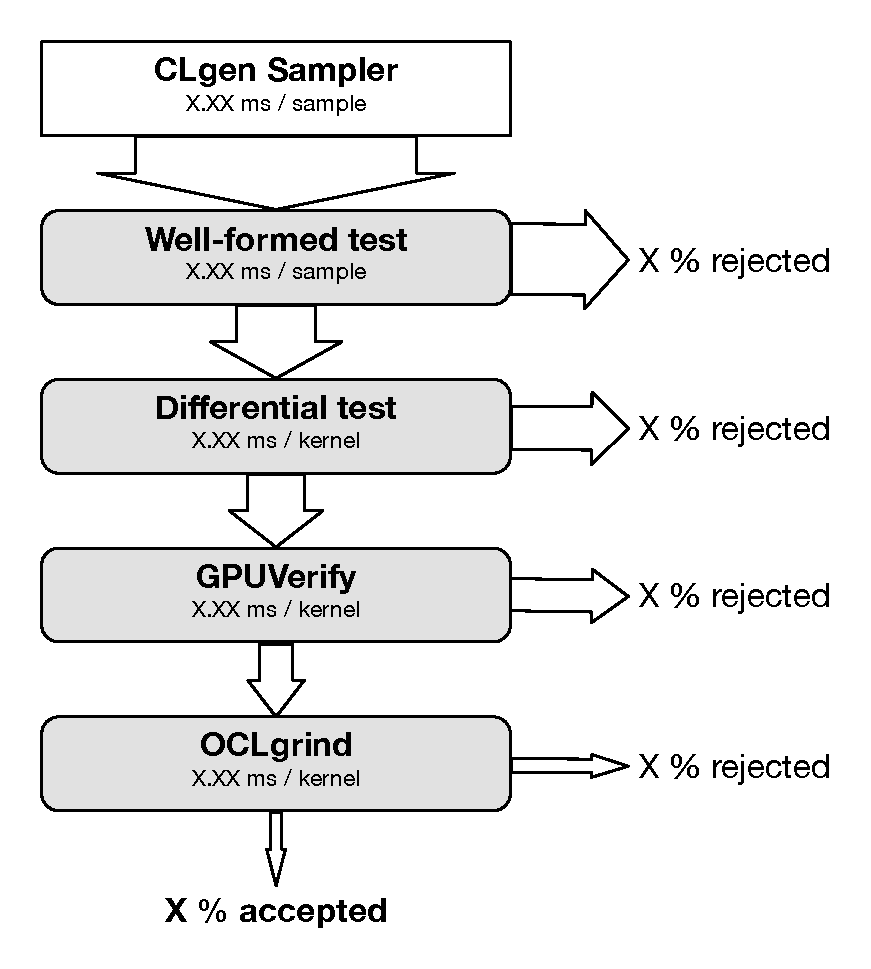
\includegraphics[width=.8\columnwidth]{img/rej} %
%         % \vspace{-2em}%
%         \caption{%
%                 Rejection pipeline.%
%         }%
%         \label{fig:deeptune}
% \end{figure}

\begin{figure}
        \centering
        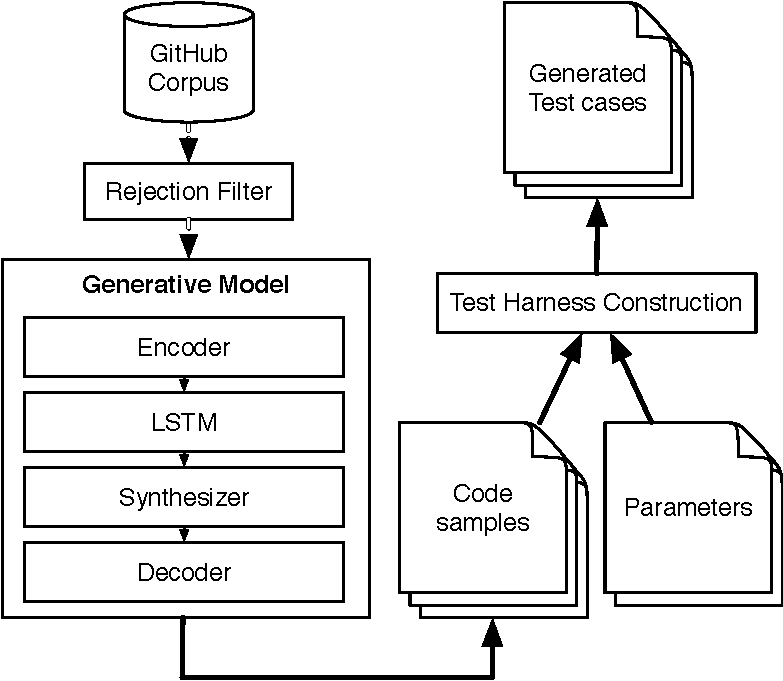
\includegraphics[width=.95\columnwidth]{img/clgen} %
        % \vspace{-2em}%
        \caption{%
                Test-case generation process. A corpus of programs from GitHub is used to seed a generative model for program codes.%
        }%
        \label{fig:deeptune}
\end{figure}

\subsection{cldrive: OpenCL Test Case Execution}

Parse AST. Read function arguments. Generate data inputs for arguments. Limited subset of data types supported: No structs, no irregular data types.


\section{Experimental Methodology} \label{sec:methodology}

\section{Experimental Results}\label{sec:results}

\subsection{Are random strings useful?}

Baseline: random string generator. We would expect badly formed CLgen samples to be more useful than random strings. If so, this confirms the hypothesis that well-formed programs are not a requirement for \emph{all} compiler testing (especially front end).
\section{Related Work}\label{sec:rw}

\paragraph{Test Case Generation}

The need to test compilers under invalid and unexpected input conditions has been long known~\cite{Boujarwah1997}.

Differential testing using test cases of ranked ``quality'' is presented in~\cite{McKeeman1998}. A lexeme generator and to test C compilers by enumerating token sequences. Similar to DeepSmith, except we weight the generation so that sequences are plausible.

Increasing complexity of generations: RandProg to CSmith. Then EMI testing, and SPE.

The \emph{fuzz taming problem} is addressed in~\cite{Chen2013}, in which a distance metric is used to rank test cases such that diverse, interesting test cases are highly ranked.

\emph{LangFuzz} attempts a similar approach of learning to generate test cases from real code~\cite{Holler2012}. For LangFuzz, the input programs are codes known to have previously exposed bugs.

Empirical comparison of compiler testing techniques~\cite{Chen2014a}

Analysis of bugs in GCC and LLVM finds 80\% of test cases to be 45 lines~\cite{Sun2016}.

\cc{TODO}~\cite{Godefroid2008a,Le2015,Sun2016a}~\cite{Kossatchev2005}.

\cc{TODO:} Directed EMI testing~\cite{Le2015}.

``As a matter of implementation quality, a compiler vendor will usually fix a segmentation fault or similar problem even if the crash-inducing test case, for example, uses a variable without initialization.''~\cite{Regehr2012a}

Skeletal program enumeration~\cite{Zhang2016a}. By enumerating entire program space, provides bounded guarantees of compiler correctness. Same shortcoming as CSmith (well formed programs only). No OpenCL implementation. Probably would take a lot of development effort. \cc{More investigation required.}

CSmith~\cite{Yang2011} and CLSmith~\cite{Lidbury2015a}. Same testing methodology, but very different design goals to our work. The explore the space of \emph{unlikely} programs, by pairing infrequently combined language features. Because Csmith programs are free form undefined behavior, there is only a single interpretation. This allows oracle-less differential testing across compilers, using a voting heuristic to identify erroneous compiler outputs. The ``shape'' of programs generated by Csmith is expert driven. The shape of programs generated by DeepSmith is data driven. The 80 probabilities which control Csmith program generation are extensively hand tuned to produce programs which ``look right''. Our data driven approach does not require this. In fact, our approach is portable across changing usage of a programming language.

The functionality of Csmith is also expert driven. Every language feature supported by Csmith must be laboriously hand crafted, and results in a very complex system of over 40,000 lines of C++ code (which still omits many language features used in real programs, like heap allocation). The language features supported by DeepSmith is bound only by those which have been used on GitHub. DeepSmith has a non-zero probability of generating programs using every language feature found on GitHub. We reason that if a language feature remains unused in the entirety of code on GitHub, then it is reasonable to assume that it is not a feature worth testing. Both Csmith and CLsmith use unrealistic safe-math macros to wrap arithmetic operations. We do not.

Both tools require test case reduction (\cite{Regehr2012a} and~\cite{Pflanzer2016}, respectively). Work in test case reduction~\cite{Regehr2012a} reduced Csmith program sizes by 74--594$\times$ while preserving the bug exposing behavior. They median reduced CSmith program size they found was only 20 lines (0.5KB).

\cc{TODO:}

EMI testing~\cite{Le2013a}, Skeletal Program enumeration~\cite{Zhang2017a}.

Fuzzing with code fragments~\cite{Holler2012}.

A mutation-based approach for the Java Virtual Machine is demonstrated in~\cite{Chena}.

TODO~\cite{White2016},~\cite{Sheridan2007}.

Grammar-base whitebox testing~\cite{Godefroid2008a}.

Our work is the first to address the challenge of generating human-like, plausible random programs.

\paragraph{GPU Testing} GPU Concurrency --- Small \emph{litmus tests}~\cite{Alglave2015}.

GPUVerify~\cite{Bardsley2014}.


\paragraph{Machine Learning} Deep Learning is a nascent field that is responsible for a multitude of breakthroughs in modeling rich, hierarchical datasets. The major milestones are reviewed in~\cite{Wang2017}, and methods in~\cite{Schmidhuber2014}.

MACHINE LEARNING FOR TESTING: Machine learning selectively unsound static analysis~\cite{Heo2017}, Learning a classifier for static analyzers~\cite{Koc2017}.
Transforming program repair ingredients with DL~\cite{White}. Program repair~\cite{Koukoutos2017a}. Learning to prioritize test programs~\cite{Chen2017}. Attention network to identify buffer overruns~\cite{Choi2016}. Localizing bugs from bug reports~\cite{Lam2016,Huo2016}.

There is an increasing interest in mining source code repositories at large scale~\cite{Allamanis2013a,White2015a,Bird2009}. Previous studies have involved data mining of GitHub to analyze software engineering practices~\cite{Wu2014,Guzman2014,Baishakhi2014a,Vasilescu2015}, for example code generation~\cite{Zhang2015a}, code summarization~\cite{Allamanis2016}, comment generation~\cite{Wong2013}, and code completion~\cite{Raychev2014}. Previous applications of deep learning to compilers have involved program synthesis for performance benchmarking~\cite{Cummins2017a} and building optimization heuristics~\cite{Cummins2017b}. No work so far has exploited mined source code for test case generation. This work is the first to do so.

\section{Conclusions}\label{sec:conclusion}

We present a novel framework for compiler fuzzing. By posing the generation of random programs as an unsupervised machine learning problem, we dramatically reduce the cost and human effort required to engineer a random program generator. Large parts of the stack are programming language-agnostic, requiring only a corpus of example programs and a test harness to target a new language.

We demonstrated our approach by targeting the challenging many-core domain of OpenCL. Our implementation, DeepSmith, has uncovered dozens of bugs in commercial and open source OpenCL implementations, covering many distinct parts of compilers. We have exposed bugs in parts of the compiler where current approaches have not, for example in missing error handling. Our test cases are small, two orders of magnitude shorter than the state-of-the-art, and easily interpretable. \cc{Something about Solidity}

%\cc{TODO:} Our future work will focus on guiding the generation of code so that, with little to no additional effort, we are able to test specific properties of interest (i.e. programs containing volatiles) or subsets of the language. 

%\cc{TODO:} Future work in targeted fuzzing. Either re-train the models on a corpus in which all programs match some property of interest (i.e. programs containing volatile), or by selective sampling to test isolated features. A grammar based implementation of that~\cite{Kusner2017} uses masking to ensure sampling only from valid production rules.



% \section{Acknowledgements}
  % double blind review


\printbibliography

\end{document}